\documentclass[fleqn,10pt]{wlscirep}
\usepackage[utf8]{inputenc}
\usepackage[T1]{fontenc}
\usepackage{lineno}
\linenumbers

\title{Twitter Sentiment Geographical Index Dataset For US in Census Level}

\author[1,2,*]{Xiaokang Fu}
\author[1]{Devika Jain}
\author[1]{Jack Hayes}
\affil[1]{Center for Geographic Analysis, Harvard University, 1737 Cambridge Street, Cambridge, 02138, US}
\affil[2]{State Key Laboratory of Information Engineering in Surveying, Mapping and Remote Sensing, Wuhan University, 129 Luoyu Road, Wuhan, 430079, China}

\affil[*]{corresponding author: Xiaokang Fu (xiaokang\_fu@fas.harvard.edu)}

% \affil[$\dag$]{these authors contributed equally to this work}


\begin{abstract}

Understanding subjective well-being (SWB) at fine geographic scales is increasingly important for policy-making and social science research. Building upon established methodologies for deriving sentiment from social media, we introduce a high-resolution Twitter Sentiment Index specifically for the United States at the census tract level. This dataset leverages deep-learning-based natural language processing techniques applied to a large corpus of geotagged tweets originating from the US from 2010 to 2023. The resulting open-source dataset provides daily, monthly, and yearly sentiment scores and tweet counts aggregated to 8.18 million US census blocks, offering unprecedented granularity for examining local variations in expressed sentiment and their potential SWB implications. This resource complements traditional survey methods by providing timely, high-frequency data suitable for studying the impacts of local events, policies, and socioeconomic conditions on public mood.

\end{abstract}
\begin{document}

\flushbottom
\maketitle

% \thispagestyle{empty}

% \noindent Please note: Abbreviations should be introduced at the first mention in the main text – no abbreviations lists or tables should be included. Structure of the main text is provided below.

\section*{Background \& Summary}


Subjective Well-Being (SWB), encompassing cognitive life evaluations and affective emotional states \cite{dienerSubjectiveWellbeing1984}, remains a critical focus for researchers and policymakers seeking measures beyond traditional economic indicators \cite{jaidkaEstimatingGeographicSubjective2020,deatonIncomeHealthWellbeing2008}. While surveys like the Gallup World Poll \cite{deatonIncomeHealthWellbeing2008} or national panels (e.g., PSID \cite{lucasMeasuringExperientialWellbeing2019}) provide valuable SWB data, they often face limitations in temporal frequency, geographic granularity, and cost \cite{chaiTwitterSentimentGeographical2023a}, particularly for tracking rapid changes or localized phenomena.

The proliferation of social media, combined with advances in Natural Language Processing (NLP), offers a complementary approach \cite{chaiTwitterSentimentGeographical2023a}. Platforms like Twitter capture real-time expressions of public mood, attitude, and feeling. Sentiment analysis techniques allow for the quantification of these expressions \cite{chaiTwitterSentimentGeographical2023a}, and studies have shown correlations between social media sentiment and survey-based SWB measures \cite{jaidkaEstimatingGeographicSubjective2020}. Previous work, including our own Twitter Sentiment Geographical Index (TSGI) \cite{chaiTwitterSentimentGeographical2023a}, demonstrated the feasibility of creating large-scale, multi-lingual sentiment indices at the country and admin-2 (county/city) levels using billions of geotagged tweets \cite{chaiTwitterSentimentGeographical2023a}. These indices have proven useful for different studies ranging from analyzing the sentiment impacts of major events like the COVID-19 pandemic \cite{wangGlobalEvidenceExpressed2022} and the complex spatial relationships between urban sprawl and SWB \cite{wangUrbanSprawlSubjective2025}, to rural–urban differences among social media users \cite{jiangRuralurbanDifferencesDeterminants2025} and global sentiment variations on decentralized finance linked to GDP per capita \cite{chenGlobalPublicSentiment2025}.

However, many social, economic, and policy dynamics occur at much finer geographic scales within countries, particularly within diverse nations like the United States. County-level aggregation can mask significant intra-county heterogeneity. To address this, we develop a new, publicly available Twitter sentiment index aggregated at the US census tract level. Census tracts are designed to be relatively homogeneous units with respect to population characteristics, economic status, and living conditions, making them a highly relevant scale for local analysis. This US Census Tract Twitter Sentiment Geographical Index (US-CT-TSGI) utilizes the same core sentiment analysis methodology as the global TSGI but applies a more granular geocoding process specific to the US administrative boundaries. This dataset provides researchers with a powerful tool to investigate neighborhood-level variations in expressed sentiment and explore their connections to local events, demographic characteristics, environmental factors, and policy interventions.

Our primary contribution is the creation of the first open-source, daily, monthly and yearly Twitter sentiment database at the US census tract level, covering  8.18 million tracts across the nation from 2010 to 2023. This dataset offers:

\begin{enumerate}
    \item High Granularity: Sentiment data resolved at the census tract level.
    \item Temporal Frequency: Daily updates enabling the analysis of short-term fluctuations
    \item Consistent Methodology: Built upon a validated BERT-based sentiment model \cite{chaiTwitterSentimentGeographical2023a}, ensuring methodological continuity with broader-scale indices.
\end{enumerate}

We anticipate this dataset will be a valuable resource for urban studies, public health, sociology, economics, and political science, enabling novel research into the micro-geographic patterns of expressed sentiment and well-being in the United States.


\section*{Methods}

% Maybe still need add more details.
% Add how we did it, but refer to previous work for more details
% like what other papers will do; maybe I will add Zifu as the co Authors, and he will be the corespnding author maybe the last author?


\subsection*{Data Collection, Cleaning and Sentiment Enhancing}


We apply the same Twitter data archive, preprocessing steps and sentiment analysis methods as detailed in our previous work \cite{chaiTwitterSentimentGeographical2023a} to ensure data quality and consistency with the sentiment model training. In addition, as we focus on the US, we utilized tweets identified as originating within the United States from XX, to XX, encompassing approximately XX billion geotagged tweets after initial filtering and cleaning.


\subsection*{Aggregating Sentiment Scores}

To ensure accurate spatial sentiment analysis at the neighborhood level, tweets were first geolocated to U.S. census blocks (the finest granularity of census geography) using TIGER/Line boundary data. Tweet-level sentiment scores (ranging from 0 to 1) were then aggregated to the census block level (identified by the 15-digit GEOID20) on daily, monthly, and yearly bases.

To account for the spatial uncertainty of tweet locations, we implemented a multi-tier aggregation strategy based on the `confidence` score derived from the spatial join process. We generated four sets of statistics for each block-time unit:
\begin{enumerate}
    \item \textbf{Strict}: Includes only tweets with a confidence score of 1.0 (exact match).
    \item \textbf{High}: Includes tweets with confidence $\ge$ 0.8.
    \item \textbf{Medium}: Includes tweets with confidence $\ge$ 0.5.
    \item \textbf{All}: Includes all tweets regardless of confidence.
\end{enumerate}

For each tier, we calculated the tweet count, unique user count, and descriptive statistics of the sentiment scores (mean, standard deviation, minimum, maximum, and percentiles: 10th, 25th, 50th, 75th, 90th). Additionally, for the 'All' tier, we computed a confidence-weighted mean sentiment score:
\[
\text{Weighted Mean} = \frac{\sum (S_i \times C_i)}{\sum C_i}
\]
where $S_i$ is the sentiment score and $C_i$ is the spatial confidence of tweet $i$.

\section*{Data Records}

The US Census Tract Twitter Sentiment Geographical Index (US-CT-TSGI) provides two levels of data: the raw spatially joined tweet archive (Table~\ref{tab:census_tgsi}) and the aggregated sentiment statistics at the census block level (Table~\ref{tab:agg_sentiment}). The datasets can be accessed at \url{XXX}.

\begin{table}[htbp]
\centering
\caption{Aggregated Sentiment Statistics Variables (Daily/Monthly/Yearly)}
\label{tab:agg_sentiment}
\begin{tabular}{llp{8cm}}
\toprule
\textbf{Variable Pattern} & \textbf{Type} & \textbf{Description} \\
\midrule
GEOID20 & String & 15-digit Census Block Identifier \\
date\_val / year / month & Date/Int & Temporal timestamp (Day, Year, or Month) \\
\{tier\}\_tweet\_count & Integer & Number of tweets in this tier (tier: strict, high, medium, all) \\
\{tier\}\_user\_count & Integer & Number of unique users in this tier \\
\{tier\}\_sentiment\_mean & Float & Mean sentiment score \\
\{tier\}\_sentiment\_std & Float & Standard deviation of sentiment scores \\
\{tier\}\_sentiment\_\{p\}q & Float & Sentiment quantiles (p $\in$ \{10, 25, 50, 75, 90\}) \\
all\_weighted\_sentiment\_mean & Float & Confidence-weighted mean sentiment score \\
all\_confidence\_mean & Float & Average spatial confidence score of tweets in the block \\
\bottomrule
\end{tabular}
\end{table}



\section*{Technical Validation}

To ensure the reliability and validity of the US-CT-TSGI dataset, we conducted a comprehensive technical validation across three dimensions: spatial representativeness, temporal stability, and external convergence with established public health indicators. Our validation relies on three external datasets: (1) block-level population counts from the 2020 US Decennial Census \cite{uscensusbureau2020decennial}, (2) TIGER/Line 2020 census tract boundary shapefiles \cite{uscensusbureau2020tigerline} for spatial visualization, and (3) the CDC PLACES dataset (2020--2024 releases) \cite{cdcplaces2024} for tract-level mental health prevalence.

\subsection*{Geographic Coverage and Representativeness}

A critical challenge in social media-based indices is the potential for geographic sampling bias. To assess this, we integrated population counts from the 2020 US Decennial Census at the block level. We calculated the Coverage Ratio (CR) for each census tract (aggregated from blocks) as follows:
\[
CR = \frac{\text{Tweet Count}}{\text{Population}}
\]
We visualize the spatial distribution of $log_2(CR)$ to identify areas of over-representation (positive values) and under-representation (negative values). Additionally, we computed the Gini coefficient and plotted the Lorenz curve to quantify the inequality of tweet distribution relative to the population.
[Insert Figure: Lorenz Curve and Gini Coefficient Result]
[Insert Figure: National Map of log2(CR)]

\subsection*{Temporal Stability and Data Consistency}

To verify the consistency of our sentiment aggregation strategy, we examined the temporal trends of tweet volumes and average sentiment scores from 2012 to 2023. We also compared the sentiment distributions derived from the 'Strict' (confidence=1.0) and 'All' tiers to ensure that including lower-confidence spatial matches does not introduce systematic bias.
[Insert Figure: Time Series Plot of Tweet Counts and Sentiment]

\subsection*{Correlation with Public Health Indicators (External Validity)}

As a measure of external validity, we examined the relationship between our Twitter-derived sentiment indices and community-level mental health outcomes. We utilized the CDC PLACES dataset (Local Data for Better Health), specifically the crude prevalence of "Mental health not good for $\ge$14 days" (MHLTH) at the census tract level.

We aggregated our block-level sentiment data to the tract level (population-weighted) for the years 2020, 2021, and 2022 to match the available CDC data. We then calculated the Pearson and Spearman correlation coefficients between the annual average sentiment scores and the MHLTH prevalence rates. A significant negative correlation would support the validity of the Twitter sentiment index as a proxy for subjective well-being.
[Insert Table/Figure: Correlation Coefficients and Scatter Plots]

\section*{Usage Notes}

% The Usage Notes should contain brief instructions to assist other researchers with reuse of the data. This may include discussion of software packages that are suitable for analysing the assay data files, suggested downstream processing steps (e.g. normalization, etc.), or tips for integrating or comparing the data records with other datasets. Authors are encouraged to provide code, programs or data-processing workflows if they may help others understand or use the data. Please see our code availability policy for advice on supplying custom code alongside Data Descriptor manuscripts.

% For studies involving privacy or safety controls on public access to the data, this section should describe in detail these controls, including how authors can apply to access the data, what criteria will be used to determine who may access the data, and any limitations on data use.

Our efforts have resulted in the development of the most extensive archive comprising two billion tweets enriched with country, state, and census-level variables. It encompasses tweet and user identification records, along with census variables, encompassing over two billion geo-tagged tweets in the U.S. from January 2012 to July 2023. As far as our knowledge extends, this dataset marks the pioneering instance of a geography-enriched tweet collection accessible at such a scale and granularity. However, our dataset has some limitations and we recommend reading this section in detail before using this dataset.

% list the limatations


\section*{Code availability}

% For all studies using custom code in the generation or processing of datasets, a statement must be included under the heading "Code availability", indicating whether and how the code can be accessed, including any restrictions to access. This section should also include information on the versions of any software used, if relevant, and any specific variables or parameters used to generate, test, or process the current dataset.

The entire source code is open-source and publicly accessible on GitHub at \url{https://github.com/wybert/US-Census-TGSI}.

\bibliography{sample}



\section*{Acknowledgements} (not compulsory)

% Acknowledgements should be brief, and should not include thanks to anonymous referees and editors, or effusive comments. Grant or contribution numbers may be acknowledged.

We extend our gratitude to Department of Government  at Harvard University for partially funding this work. We would like to thank Harvard FAS Research Computing for providing the technical support and computing resources needed for the project. We would also like to thank Heavy.ai for providing us the software license to their product.


\section*{Author contributions statement}

Must include all authors, identified by initials, for example:
A.A. conceived the experiment(s), A.A. and B.A. conducted the experiment(s), C.A. and D.A. analysed the results. All authors reviewed the manuscript.

\section*{Competing interests} (mandatory statement)

% The corresponding author is responsible for providing a \href{https://www.nature.com/sdata/policies/editorial-and-publishing-policies#competing}{competing interests statement} on behalf of all authors of the paper. This statement must be included in the submitted article file.

All authors declare that they have no conflicts of interest. Authors used ChatGPT 4 in order to improve readability and language.


\section*{Figures \& Tables}

% Figures, tables, and their legends, should be included at the end of the document. Figures and tables can be referenced in \LaTeX{} using the ref command, e.g. Figure \ref{fig:stream} and Table \ref{tab:example}.

% Authors are encouraged to provide one or more tables that provide basic information on the main ‘inputs’ to the study (e.g. samples, participants, or information sources) and the main data outputs of the study. Tables in the manuscript should generally not be used to present primary data (i.e. measurements). Tables containing primary data should be submitted to an appropriate data repository.

% Tables may be provided within the \LaTeX{} document or as separate files (tab-delimited text or Excel files). Legends, where needed, should be included here. Generally, a Data Descriptor should have fewer than ten Tables, but more may be allowed when needed. Tables may be of any size, but only Tables which fit onto a single printed page will be included in the PDF version of the article (up to a maximum of three).

% Due to typesetting constraints, tables that do not fit onto a single A4 page cannot be included in the PDF version of the article and will be made available in the online version only. Any such tables must be labelled in the text as ‘Online-only’ tables and numbered separately from the main table list e.g. ‘Table 1, Table 2, Online-only Table 1’ etc.

% \begin{figure}[ht]
% \centering
% 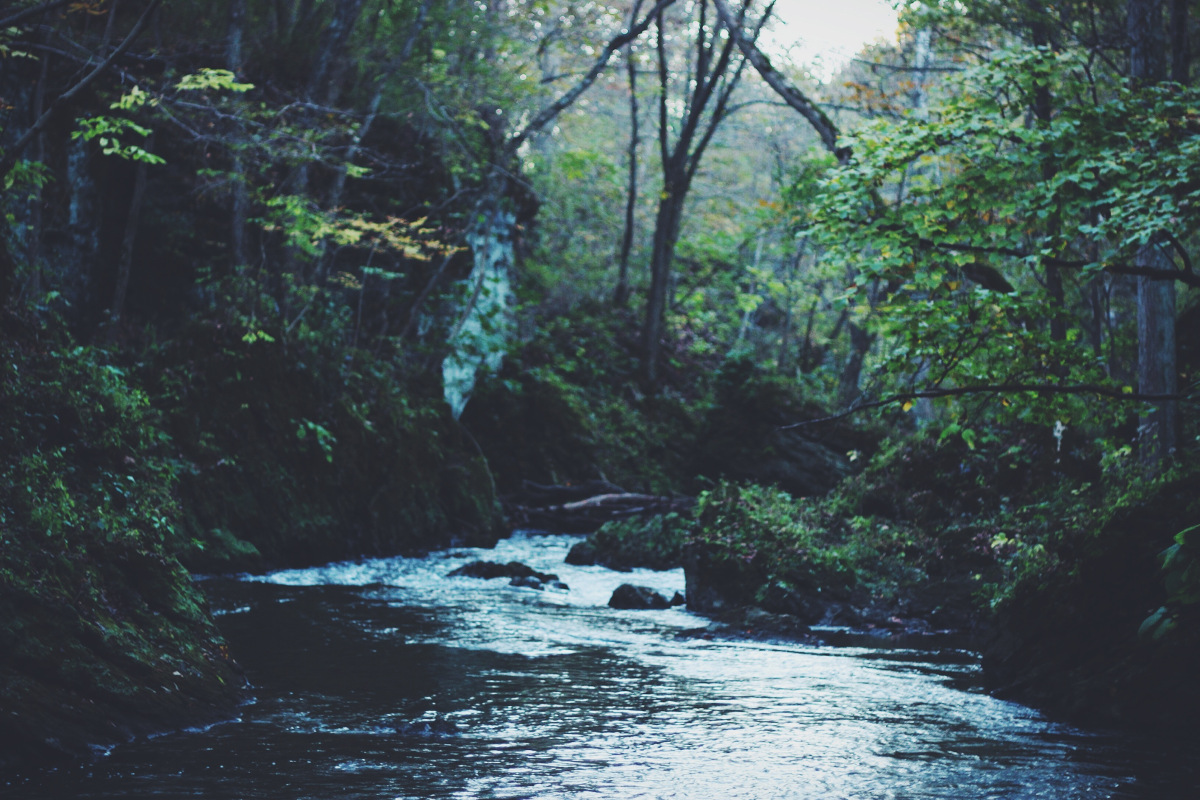
\includegraphics[width=\linewidth]{stream}
% \caption{Legend (350 words max). Example legend text.}
% \label{fig:stream}
% \end{figure}

% \begin{table}[ht]
% \centering
% \begin{tabular}{|l|l|l|}
% \hline
% Condition & n & p \\
% \hline
% A & 5 & 0.1 \\
% \hline
% B & 10 & 0.01 \\
% \hline
% \end{tabular}
% \caption{\label{tab:example}Legend (350 words max). Example legend text.}
% \end{table}

% \begin{figure}[ht]
%     \centering
%     \includegraphics[scale=0.6]{figures/method.drawio.pdf}
%     \caption{Workflow to merge the geotagged tweets with administrative boundaries.}
%     \label{fig:method}
% \end{figure}

% \begin{figure}[ht]
%     \centering
%     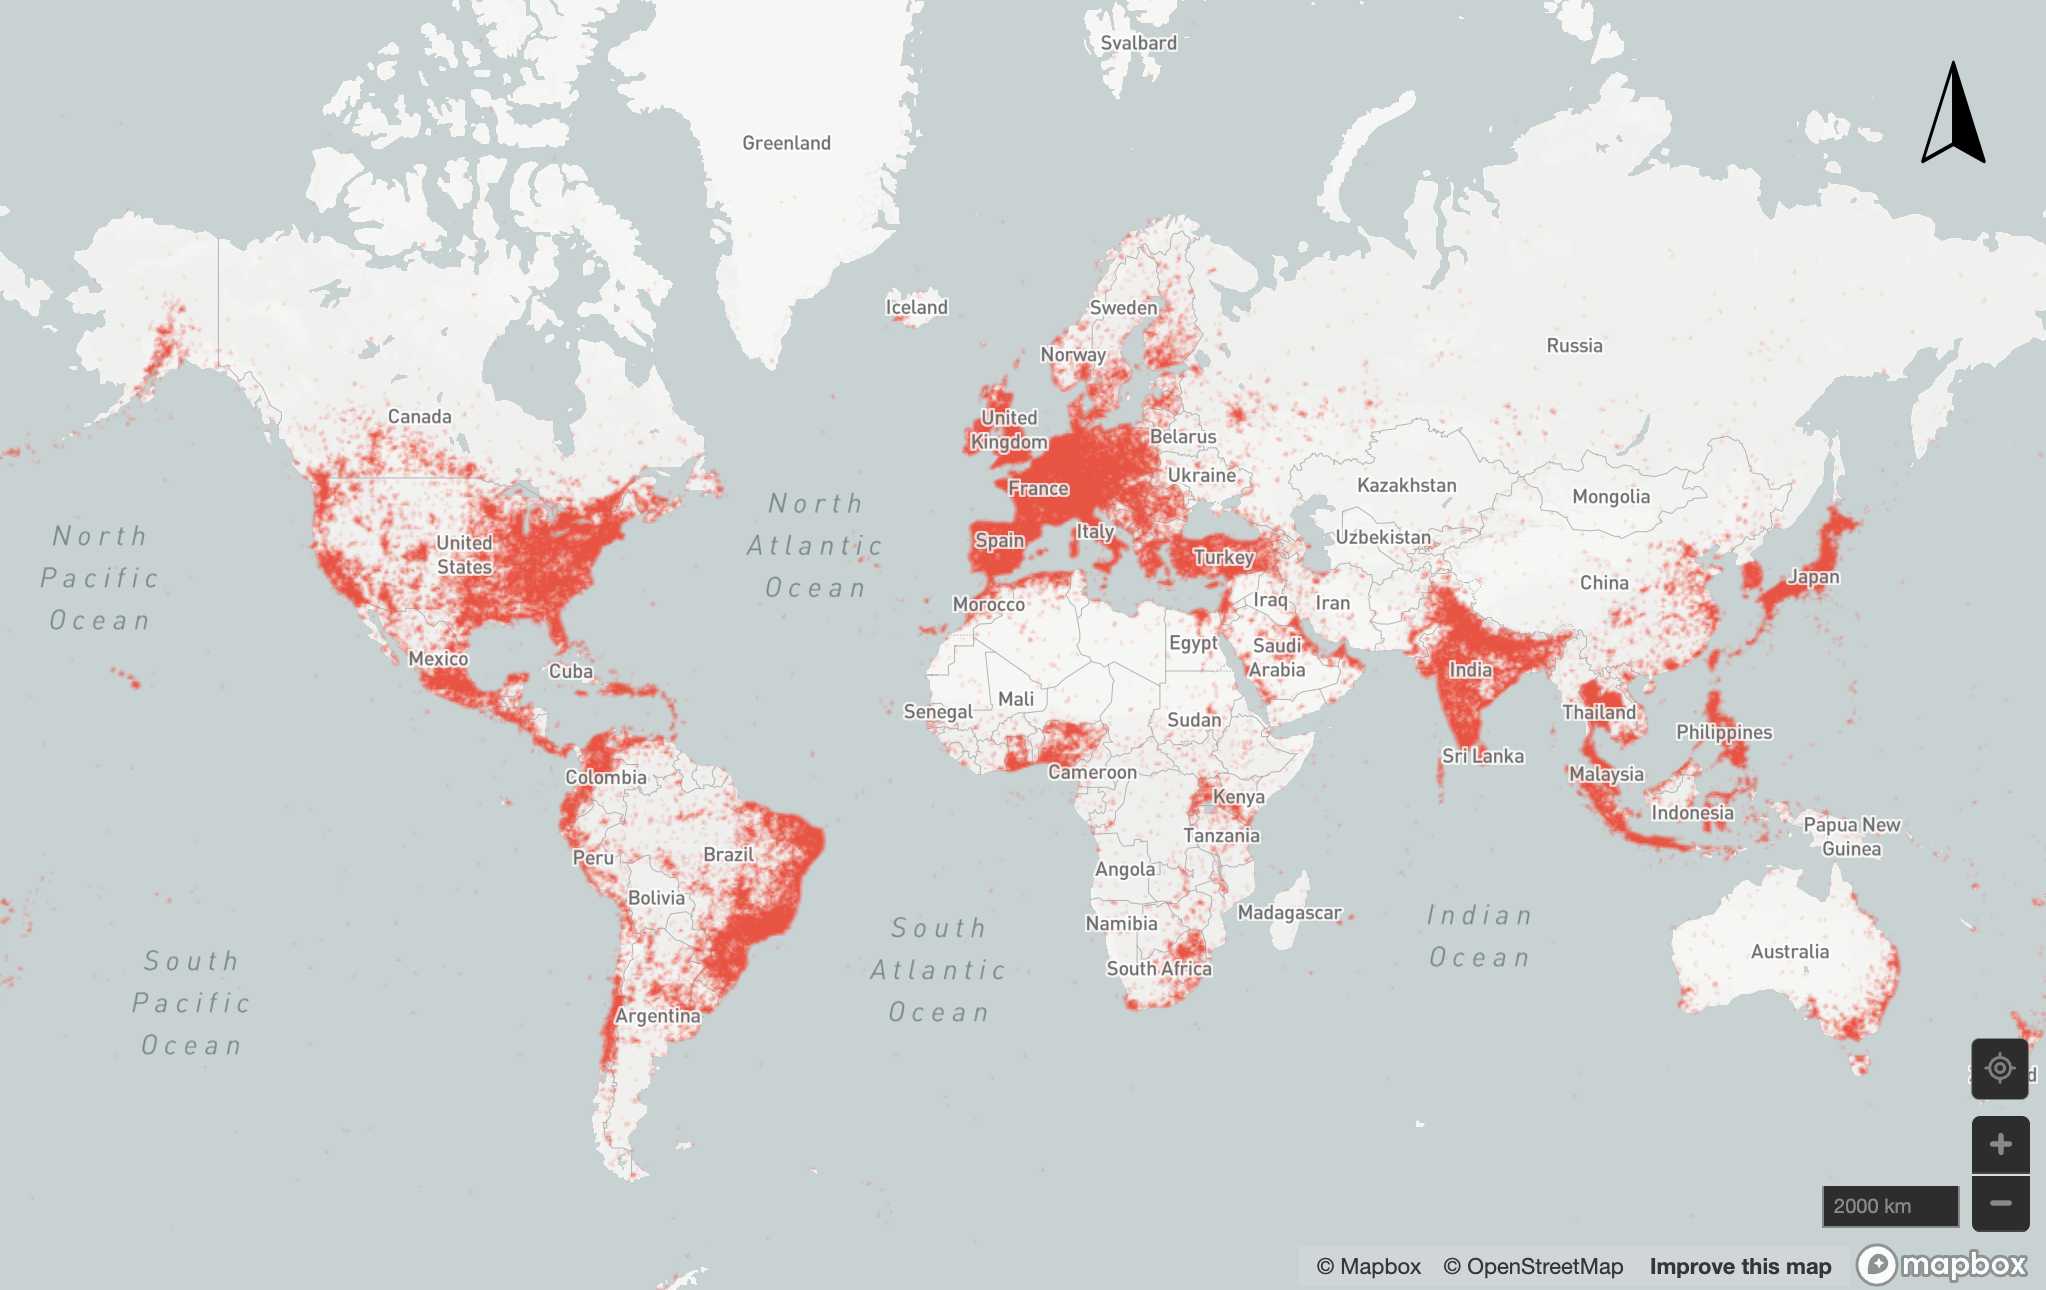
\includegraphics[scale=0.15]{figures/tweets_north_arrow.png}
%     \caption{Spatial distribution of the Geotweets from Jan 1, 2023 to Feb 28, 2023, generated by using Heavy Immerse.}
%     \label{fig:tweets_distribution}
% \end{figure}

% \begin{figure}[ht]
%     \centering
%     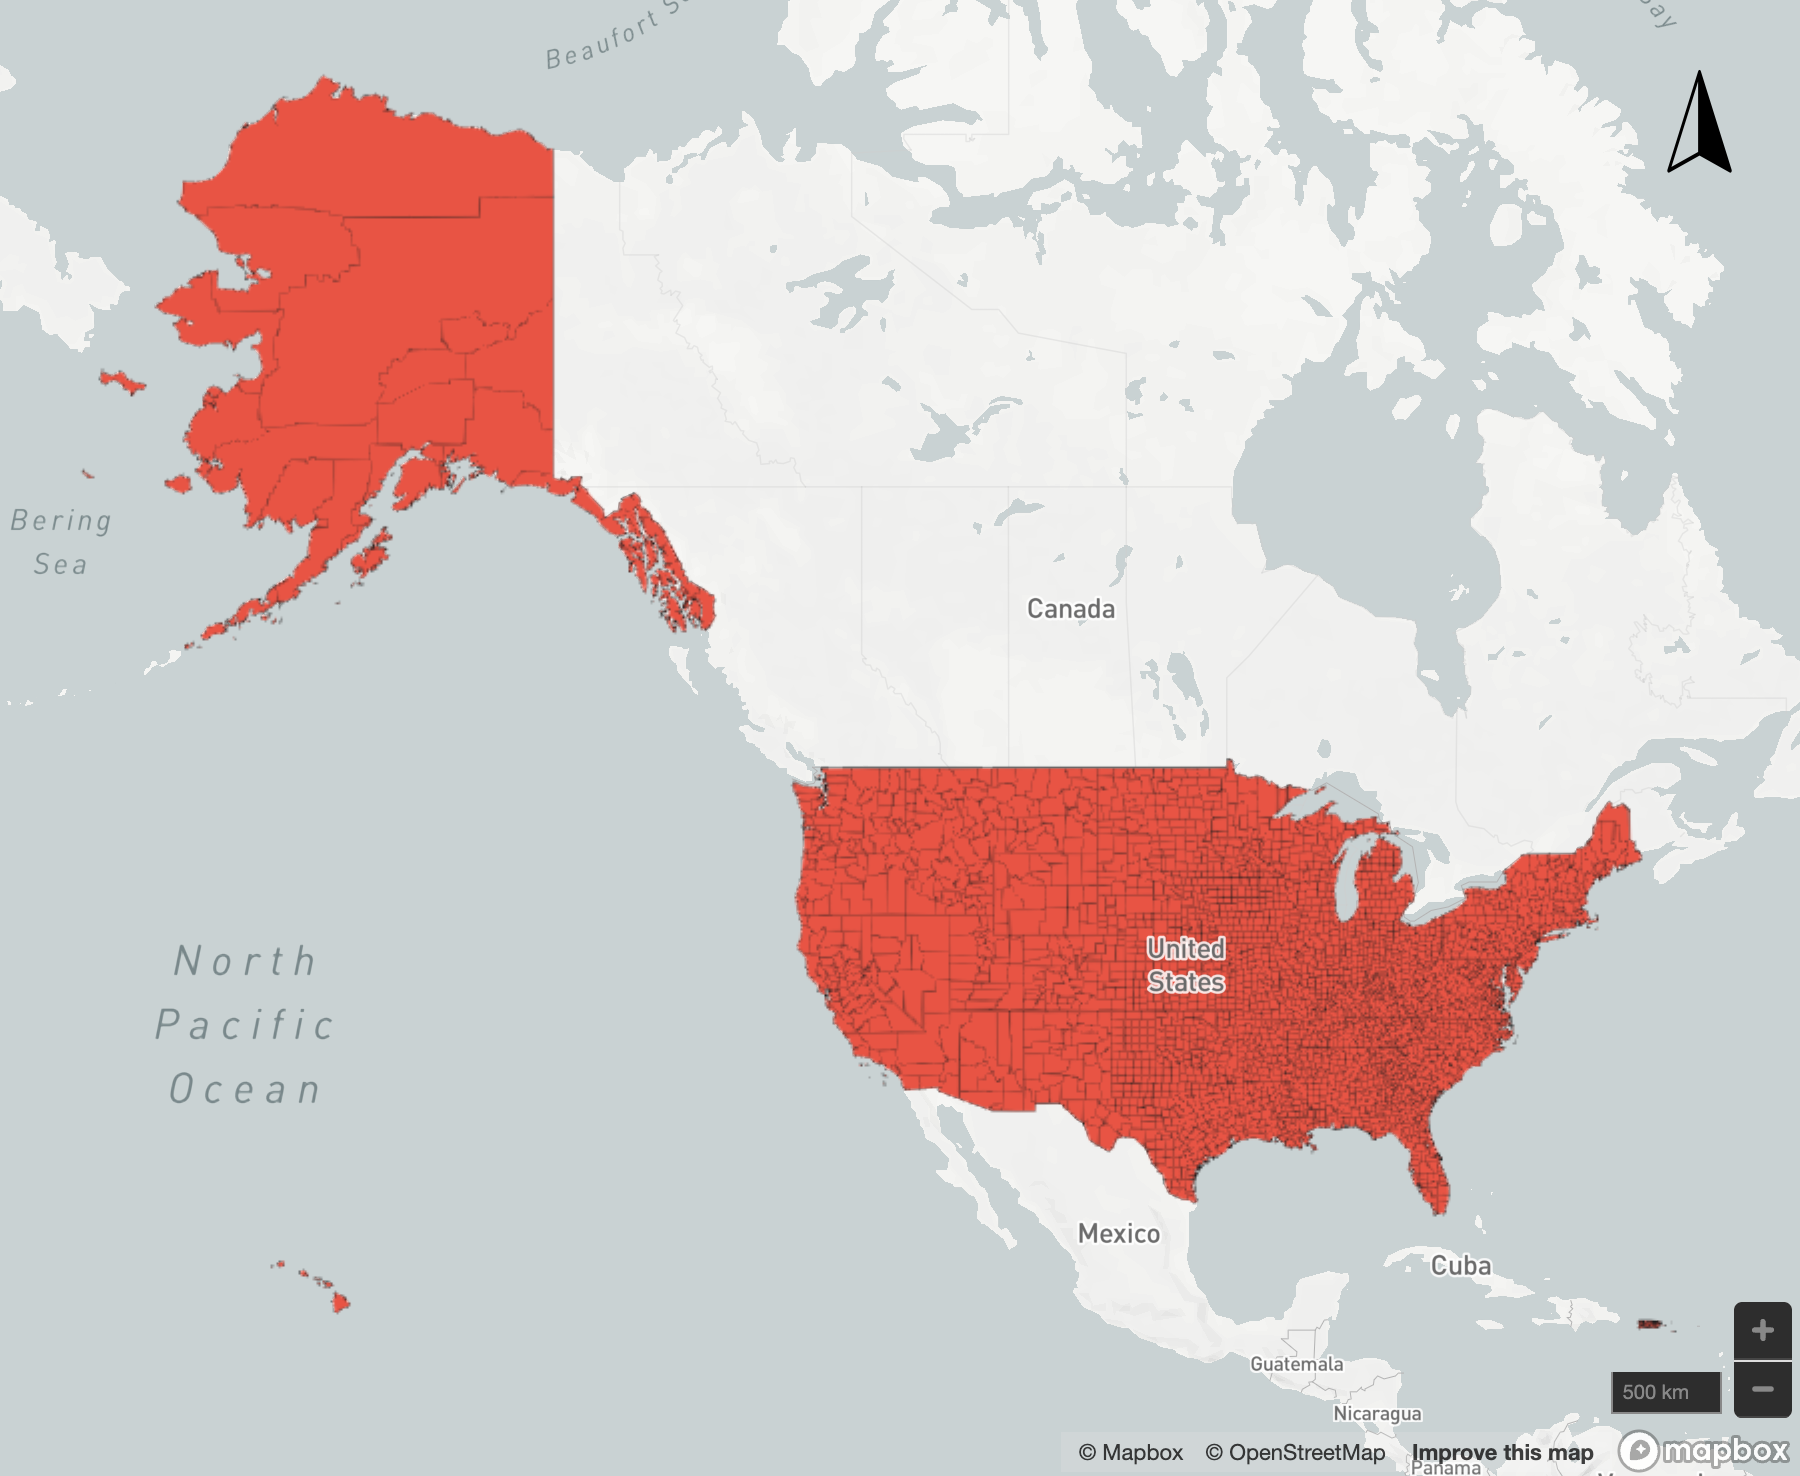
\includegraphics[scale=0.15]{figures/us_county_north.png}
%     \caption{US County Boundaries.}
%     \label{fig:us_boundaries}
% \end{figure}

% FIXME: FIX the table here
\begin{table}[htbp]
\centering
\caption{Geotweet Census Archive}
\label{tab:census_tgsi}
\begin{tabular}{llp{8cm}}
\toprule
\textbf{Entry} & \textbf{Variable} & \textbf{Description} \\
\midrule
1 & message\_id & Tweet ID \\
2 & user\_id & User ID number \\
3 & fips & County FIPS code \\
4 & county & County name \\
5 & state & State abbreviation \\
6 & GEOID20 & Census block GEOID \\
7 & sentiment\_score & Sentiment score (0--1) calculated using BERT model \\
\bottomrule
\end{tabular}
\end{table}


\begin{table}[htbp]
\centering
\caption{Census Block Variables}
\label{tab:census_block}
\begin{tabular}{llp{8cm}}
\toprule
\textbf{Entry} & \textbf{Variable} & \textbf{Description} \\
\midrule
1 & STATEFP20 & 2020 Census state FIPS code \\
2 & COUNTYFP20 & 2020 Census county FIPS code \\
3 & TRACTCE20 & 2020 Census tract code \\
4 & BLOCKCE20 & 2020 Census tabulation block number \\
5 & GEOID20 & Census block identifier; a concatenation of 2020 Census state FIPS code, 2020 Census county FIPS code, 2020 Census tract code, and 2020 Census block number \\
6 & GEOIDFQ20 & 2020 Fully Qualified GEOID \\
7 & NAME20 & 2020 Census tabulation block name; a concatenation of ‘Block’ and the tabulation block number \\
8 & MTFCC20 & MAF/TIGER Feature Class Code (G5040) \\
9 & UR20 & Reserved for 2020 Census urban/rural indicator (2020 Urban Areas are not yet defined) \\
10 & UACE20 & Reserved for 2020 Census urban area code (2020 Urban Areas are not yet defined) \\
11 & FUNCSTAT20 & 2020 Census functional status \\
12 & ALAND20 & 2020 Census land area \\
13 & AWATER20 & 2020 Census water area \\
14 & INTPTLAT20 & 2020 Census latitude of the internal point \\
15 & INTPTLON20 & 2020 Census longitude of the internal point \\
16 & HOUSING20 & 2020 Housing Unit Count \\
17 & POP20 & 2020 Population \\
\bottomrule
\end{tabular}
\end{table}

\end{document}
